\chapter{Basics of Word2Vec and Echo State Network}\label{basics}

\section{Word2Vec}

Word2vec is a neural probalistic language model based on Distributional Hypothesis which states that the words that appears in the same context share the semantic meaning \cite{w2v:tensor_flow}. The proposed by Mikolov et al. \cite{w2v:mikolov_2013_distributed}, which takes in input a large text data to generate the distributed word  embedding of the words present in text and also preserve the linear regularities among words. In other words, it maps the words into a continuous vector space where semantically related words are placed closed to each other in the vector space. Earlier the words have been treated as discrete atomic symbols in all traditional NLP system, where each word were represented in a localist fashion. Localist representation of words does not contain any semantic or syntactic information of the word it is encoding and thus depriving the NLP systems to utilize this information while processing \cite{w2v:baroni:2014}. Word2vec neural word embeddings overcomes this issue and capture the semantics and syntactic information of the word in a computationally-efficient manner \cite{w2v:mikolov_2013_efficient}. For learning word embedding two neural architecture were proposed, the Continuous Bag Of Word (CBOW) and Skip-Gram (SG) \cite{w2v:mikolov_2013_efficient, w2v:mikolov_2013_distributed}. Both the models are architecturally same i.e. both have three layers, the input layer, hidden layer and an output layer, but have different training objectives. The architecture of both CBOW and SG models is shown in figure \ref{fig:cbow} and \ref{fig:sg} respectively. In the next sections we give a brief overview of CBOW model and SG model. However we used skip-gram model in our work because it was proven that it produce better word-embeddings as compared to CBOW \cite{w2v:mikolov_2013_distributed}.

\begin{figure}[hbtp]
\centering
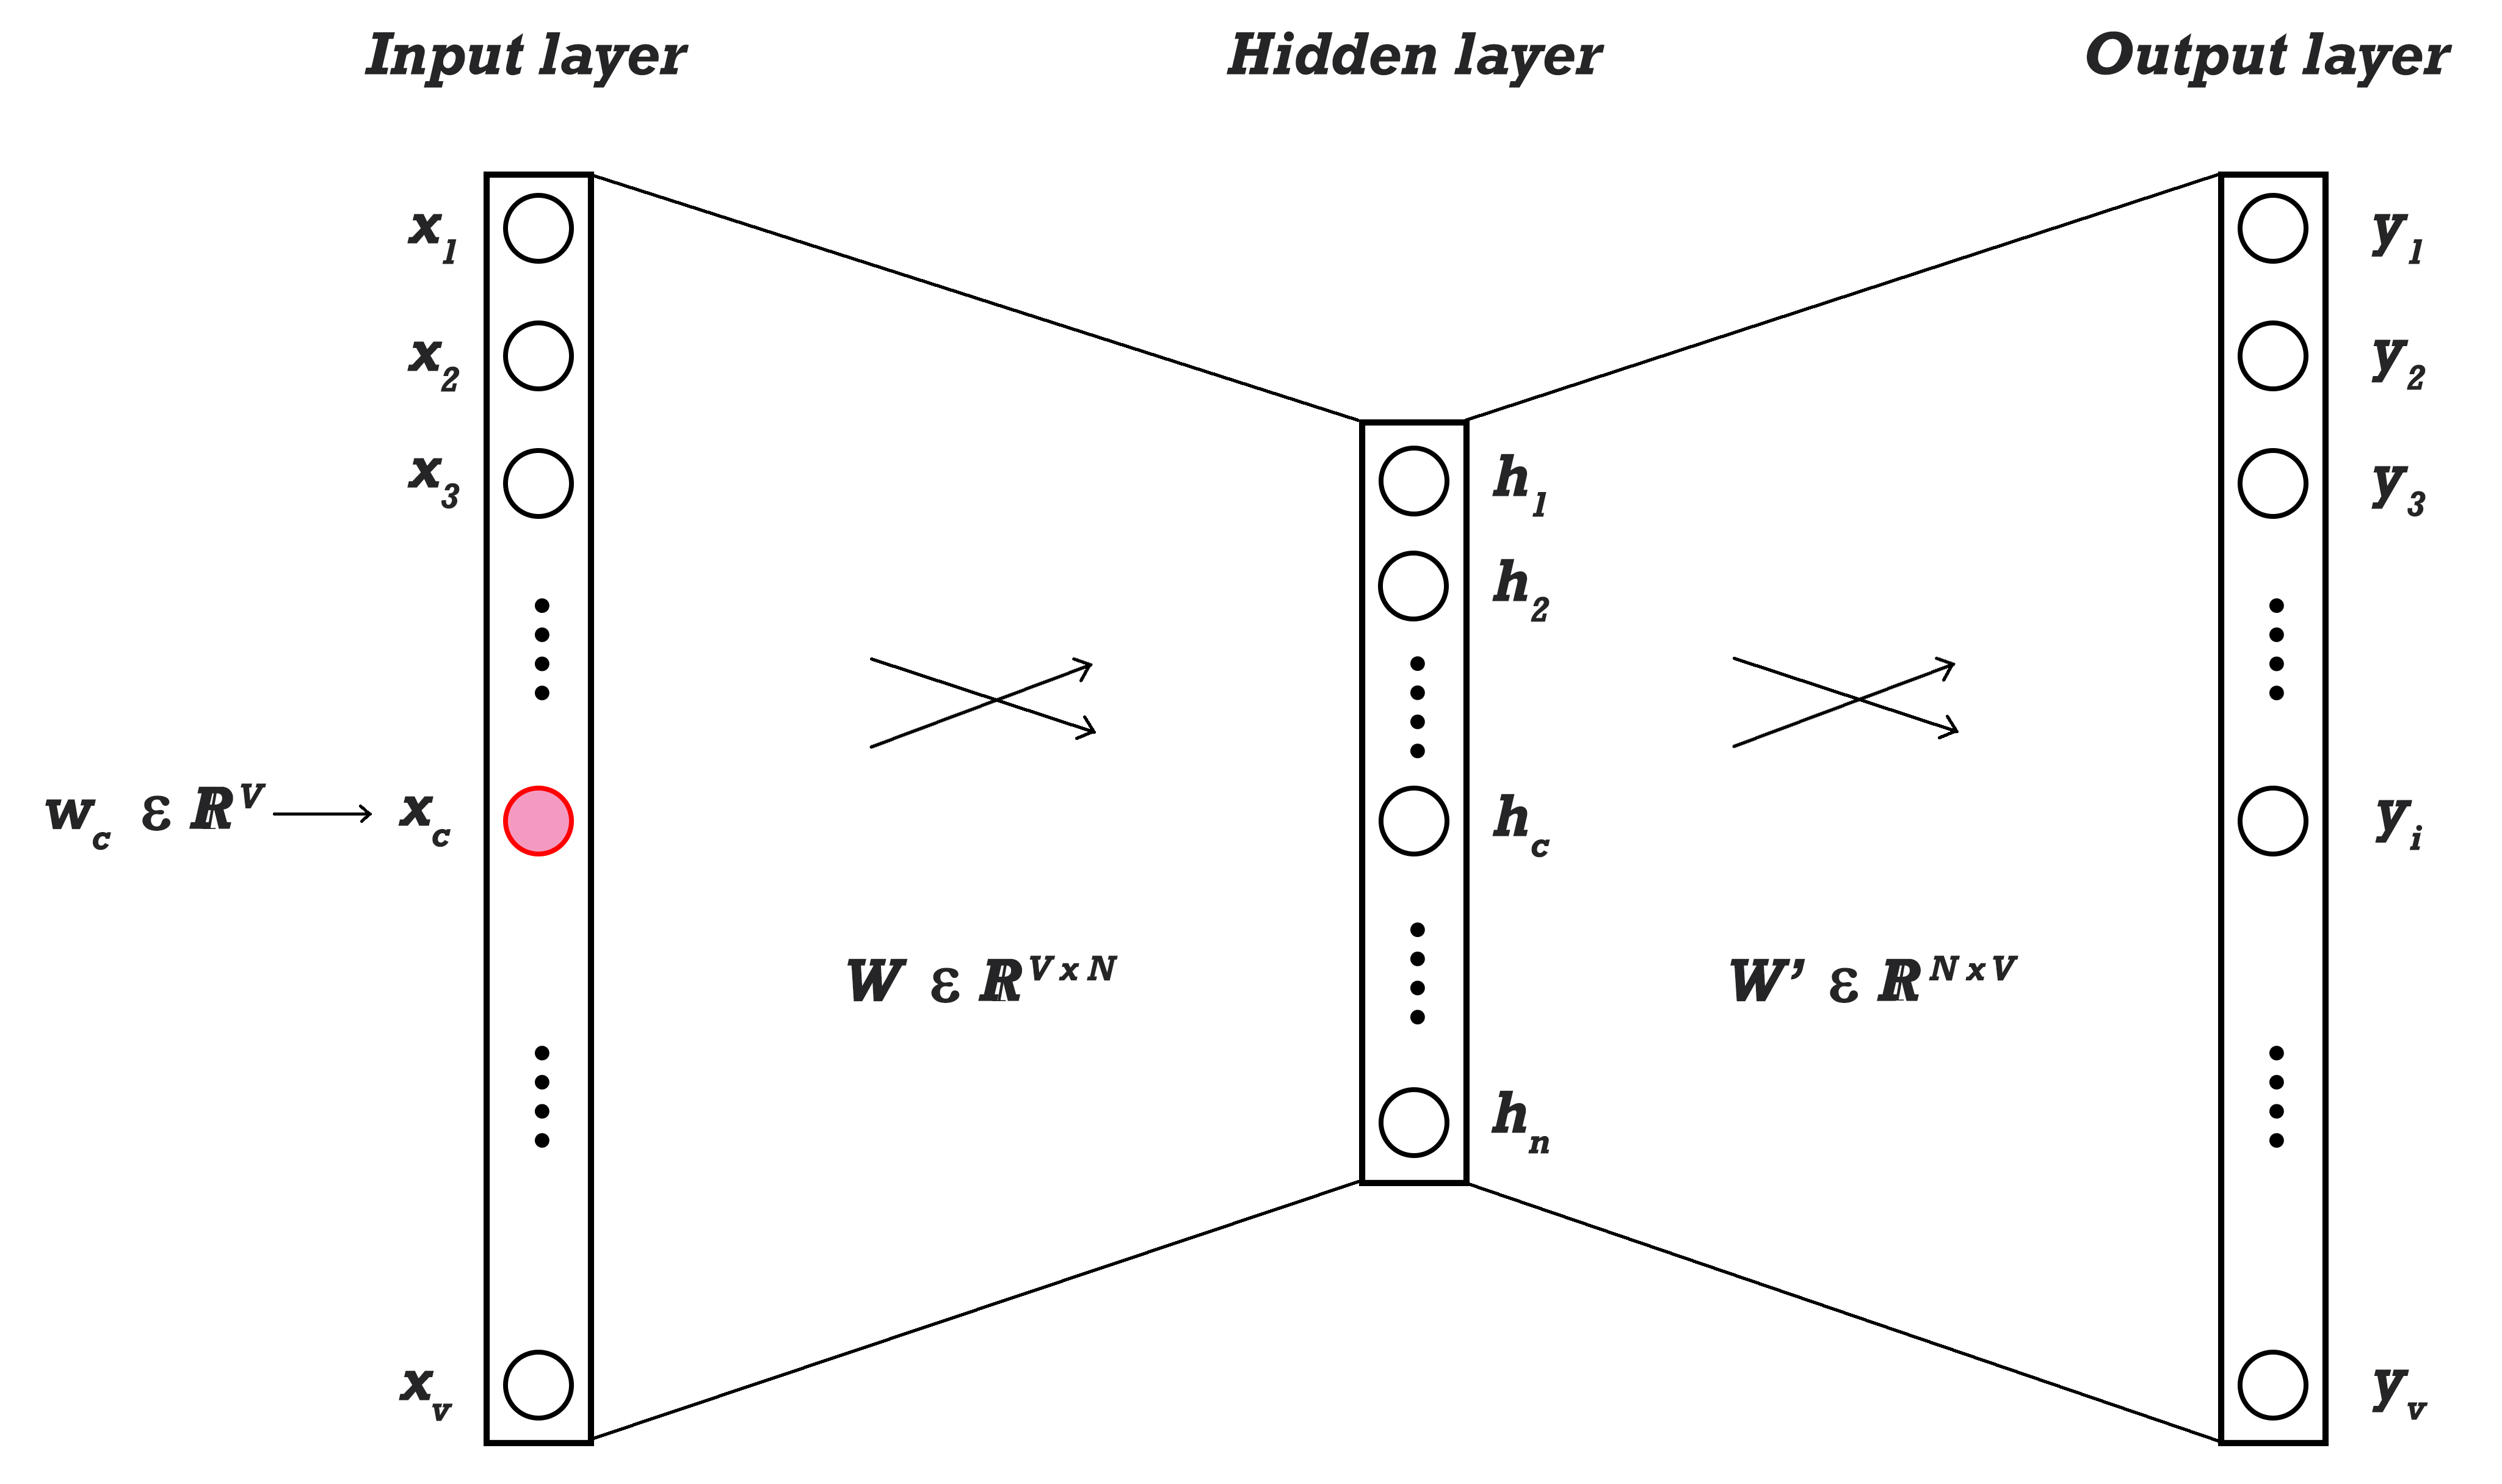
\includegraphics[width=0.8\linewidth,height=10cm,keepaspectratio]{cbow}
\caption[The CBOW model]{\textbf{The CBOW model: } In the CBOW model, the objective is to predict the target word from the words in the context (or neighbouring words). The context words are input to the model (in this case only one) using localist representation where only one vector element corresponding to input word is active ($x_{c}$, shown in red). The model outputs the probability for each word in vocabulary, which is maximized for actual target word during training. Adapted from [ref].}
\label{fig:cbow}
\end{figure}

\begin{figure}[hbtp]
\centering
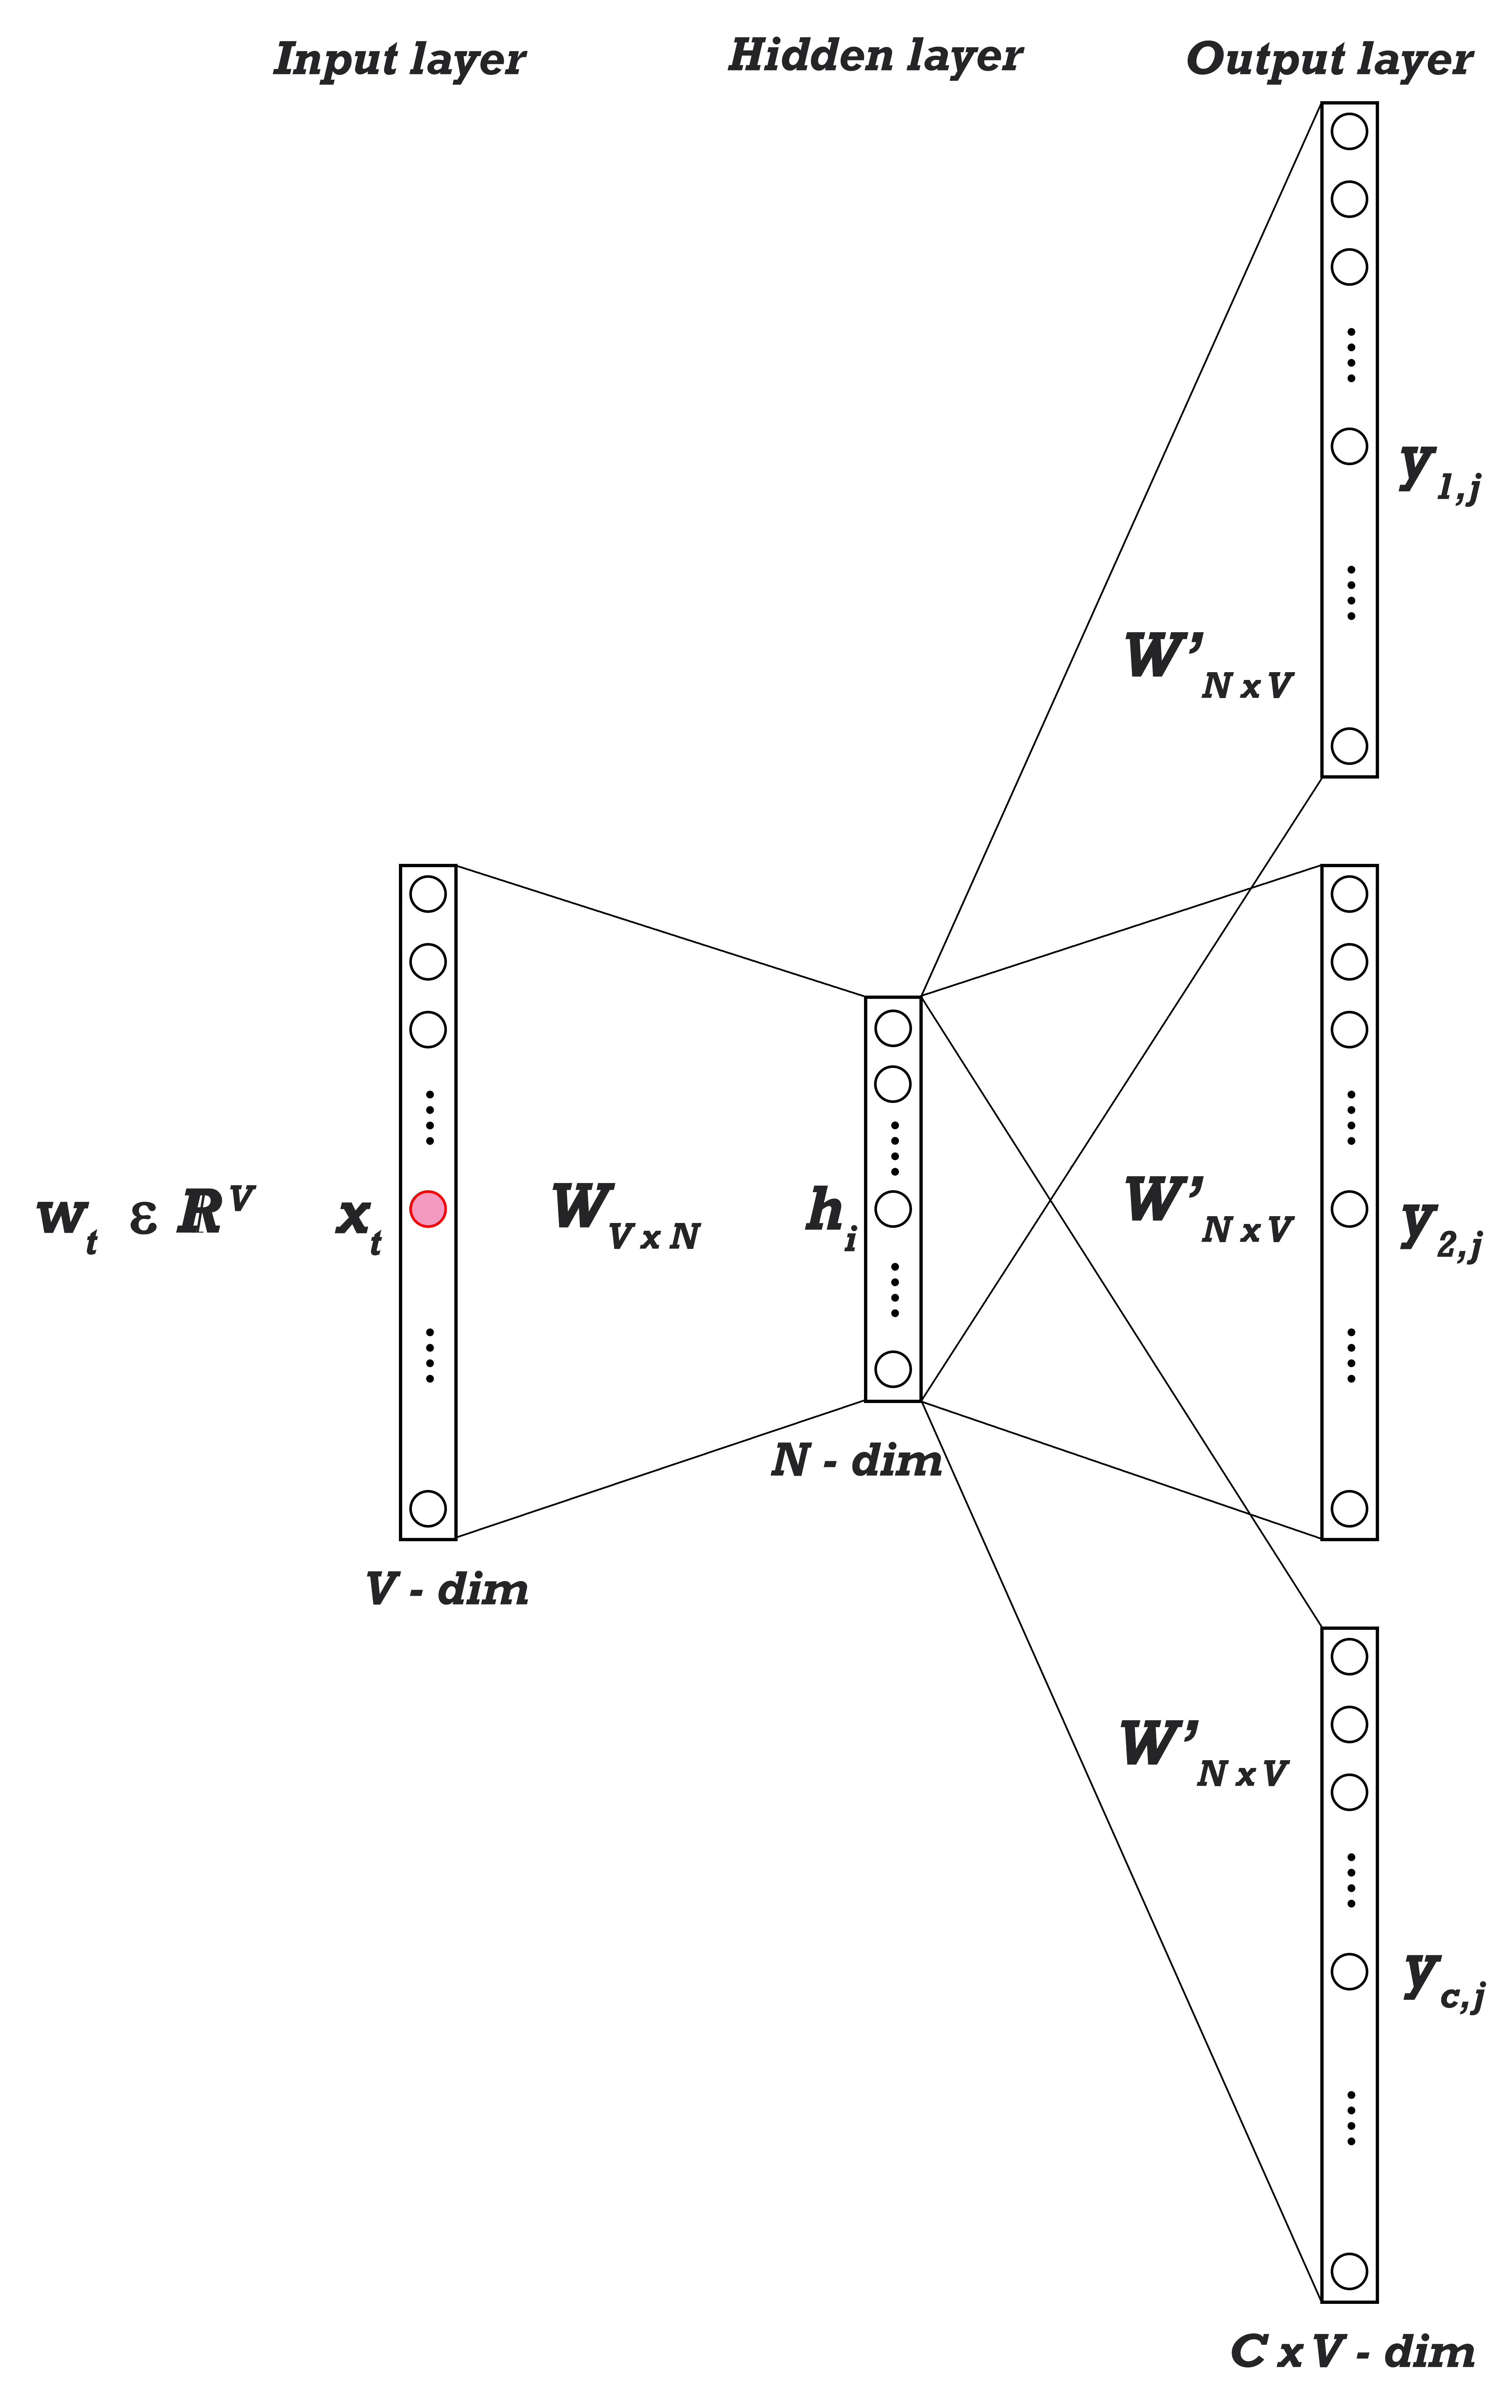
\includegraphics[width=1.8\linewidth,height=10cm,keepaspectratio]{sg}
\caption[The Skip-gram model]{\textbf{The skip-gram model: }In the skip model, the objective is reverse of CBOW. It predict the context words from the word. The target word is input to the model using localist representation where only one vector element corresponding to input word is active ($x_{t}$, shown in red). The model then maximizes the probaility of context words during training. Adapted from [ref].}
\label{fig:sg}
\end{figure}

\subsection{CBOW Model}

CBOW  model is a three layered neural model with the training objective to predict a target word (e.g. Peter) given some context words (John gave ball to …). Figure \ref{fig:cbow} shows the CBOW network architecture with a simplified case of one context word. The model is trained on the dataset having a vocabulary size $V$ in an unsupervised way to achieve the objective. The hidden layer is of size $N$, the dimensions of desired word embedding, and neurons in both the adjacent layer i.e. input and output layers,  are fully connected to hidden layer neurons. The input to the network is the context word $w_c {\in} \mathbb{R}^{V}$ and is represented using localist representation where only one unit $x_c$ at index c will be 1 out of V units $w_c=[{x_1,.....,x_V}]$ and all other units will be 0 \cite{w2v:parameter_learning}. The activation of hidden layer is then given by :

\begin{equation}\label{eqn:hidden_act}
	h = W^T . w_c= W_{(c,:)}=v_{c}
\end{equation}

where $W {\in} \mathbb{R}^{V{\times}N}$ is the weight matrix from input to hidden layer and $v_{c}$ is the vector embedding of the context word $w_c$. Eqn. \ref{eqn:hidden_act} basically copies the $c^{th}$ row of weight matrix $W$ on the hidden layer as hidden layer activation function is linear. 

A score $u {\in}\mathbb{R}^V$ is then calculated for all the target words in the vocabulary, which is essentially the compatibility of a word $w_i$ given the context word $w_c$.

\begin{equation}
\begin{split}
		 u &={W^{'}} ^ T . h \\
	   	   &= {W^{'}}^T. v_{c}	
\end{split}
\end{equation}

\begin{equation}
	u_i = {W^{'}_i}^T. v_{c}
\end{equation}

\noindent  where $u_i$ gives the score of $i^{th}$ word,$w_{i}$, for i = 1, 2...V. $W^{'}{\in} \mathbb{R}^{N{\times}V} $ is the weight matrix between hidden and output layer. ${W^{'}_i}$ is the $i^{th}$ column vector of matrix $W^{'}$.  
The computed scores are then converted to posterior probabilities by output neurons with softmax activation function. Thus aliasing ${W^{'}_i}$ as $v^{'}_{i}$ we get output probabilities as: 

\begin{equation}
\begin{split}	
y_i &= P(w_i | w_c) = \frac {\exp(u_i)} {\sum_{i' {\in} V} \exp (u_{i^{'}})}\\
	&= \frac {\exp({v^{'}_{i}}^T.v_{c})}{\sum_{i' {\in} V}\exp({v^{'}_{i^{'}}}^T.v_{c})}
\end{split}
\end{equation}
where $y_i$ is the probability of $i^{th}$ word given the context word.

The training objective is then achieved by maximizing the log likelihood of actual target word $(w_{t})$ given the context word ($w_{c}$). So the cost functions can be written as:

\begin{equation}
  \begin{split}
  	J_{ML} &= max \log P(w_t | w_c) \\
		   &= {v^{'}_{t}}^T.v_{c}- \text{ log} \sum_{i' {\in} V} {\exp({v^{'}_{i^{'}}}^T.v_{c})}
  \end{split}
\end{equation} 

In case of multiple context words is input to the network, the equation \ref{eqn:hidden_act} only change to:

\begin{equation}
h= \frac {1}{K} .(v_{c_1}+v_{c_2}+.......+v_{c_K}) 
\end{equation}	

where $k$ is the size of context window. This equation averages vector embeddings of all context words \cite{w2v:parameter_learning}.

\subsection{Skip-gram Model}

In the Skip-Gram model training objective is reversed from that of CBOW model. In other words, the objective is to learn the vector representation of the word that is good in predicting the context words \cite{w2v:mikolov_2013_distributed}. Thus for a given sequence of words $\{w_1,.....w_V\}$, the objective is to maximize the average log probability. 

\begin{equation}
\frac {1}{V}\sum_{t=1}^{V} \sum_{{-c \leq j \leq c},{j \neq 0}} {log\ P(w_{t+j}|w_t)}
\end{equation}

where c is the size of context window, $P(w_{t+c}|w_t)$ is the probability of context word $w_{t+j}$ for $-c \leq j \leq c$, given the target word $w_t$. This is measured using softmax function as:

\begin{equation} \label{eqn:sg_prob}
p(w_{t+j}|w_t)=\frac {\exp({{v^{'}_{t+j}}^{T}}.{v_t})}{\sum_{w {\in}V} \exp({{v^{'}_{w}}^{T}}.{v_t})}
\end{equation}

\noindent where ${v^{'}_{t+j}}$ and ${v_t}$ are the vector representation of word $w_{t+j}$ and $w_{t}$ respectively.

The objective function is thus optimized using stochastic gradient descent to learn the good word vectors. Calculating the full softmax is computationally expensive as it need to compute and normalize probability for every other word $w$ in the vocabulary V for a given input word ($w_{c}$ for CBOW or $w_{t}$ for skip-gram) at every training step. Thus negative sampling was proposed for learning the word embeddings\cite{w2v:mikolov_2013_distributed}.

\subsubsection{Skip-gram with negative sampling}

For learning word features full probabilistic models was not required. So in skip-gram negative sampling is used for approximation of word features. This technique treats feature learning as a binary classification (logistics regression) problems \cite{w2v:mikolov_2013_distributed, w2v:tensor_flow}. The model is thus trained to distinguish the target word from $k$ imaginary noise words $w_{noise}$, in the same context. Thus the log probability $p(w_{t+j}|w_t)$ in equation \ref{eqn:sg_prob} is now approximated by:

\begin{equation}
p(w_{t+j}|w_t)=log\ \sigma({{v^{'}_{t+j}}^{T}}.{v_t})\ +\  \sum_{w_{noise}{\in}N_{k}} \log\ \sigma({{v^{'}_{noise}}^T}.v_{t})
\end{equation}

\noindent where $\sigma(x)=1/(1+\exp(-x))$, and $N_k$ is the set of $k$ noise word compared to corresponding context word $w_{t+j}$ for $-c \leq j \leq c$. 

\subsection{Properties of Word2Vec embeddings}

Although the word2vec model is simple in architecture and easy to train, it produces word vector embedding which surprisingly encodes several linguistic regularities and patterns \cite{w2v:language_similarities, w2v:mikolov_2013_distributed}. More importantly it is astonishing because the network was not explicitly trained for these linguistic properties (see fig. \ref{fig:sem_rel} and \ref{fig:w2v_translation}). The distributed word embeddings encodes semantic and syntactic properties of the words as a constant vector offset between a pair of words sharing a specific relationship\cite{w2v:mikolov_2013_distributed}. For example, the word embeddings $"King - Queen \approx man - woman"$, $"apples - apple \approx cars - car"$, $"walking - walked \approx swimming - swam"$.

\begin{figure}[hbtp]
\centering
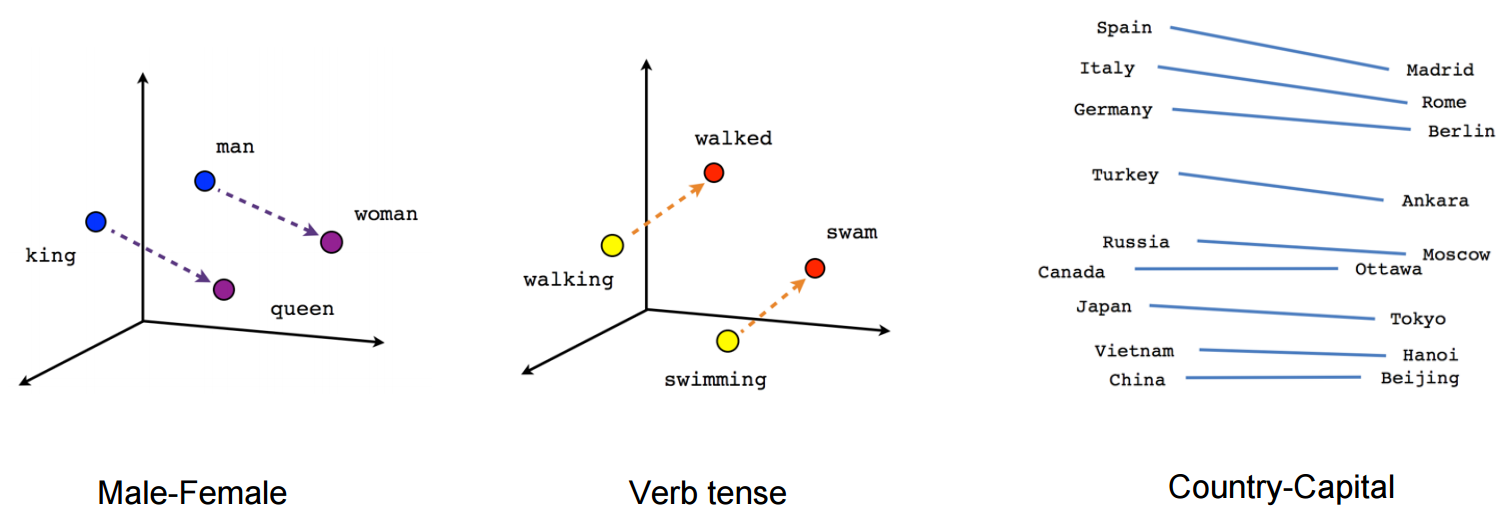
\includegraphics[width=0.8\linewidth]{linear-relationships}
\caption[Word2vec semantic regularities]{\textbf{Word2vec semantic regularities.}} 
\label{fig:sem_rel}
\end{figure}

\begin{figure}[hbtp]
\centering
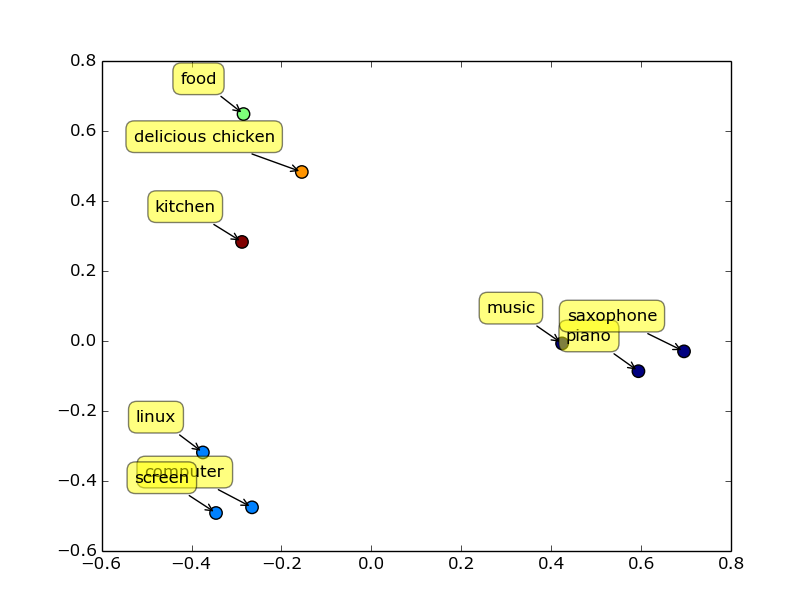
\includegraphics[width=0.8\linewidth]{word2vec_clustering}
\caption [Word2Vec word clustering]{\textbf{Word Clustering with word2vec word embedding:} The figure shows the word clustering property obtained by projecting the word vectors on two dimesional space using PCA. The words vector taken from pretrained word2vec Google News corpus\footnotemark }
\label{fig:w2v_clustering}
\end{figure}

\footnote{https://drive.google.com/file/d/0B7XkCwpI5KDYNlNUTTlSS21pQmM/edit}

\begin{figure}[hbtp]
\centering
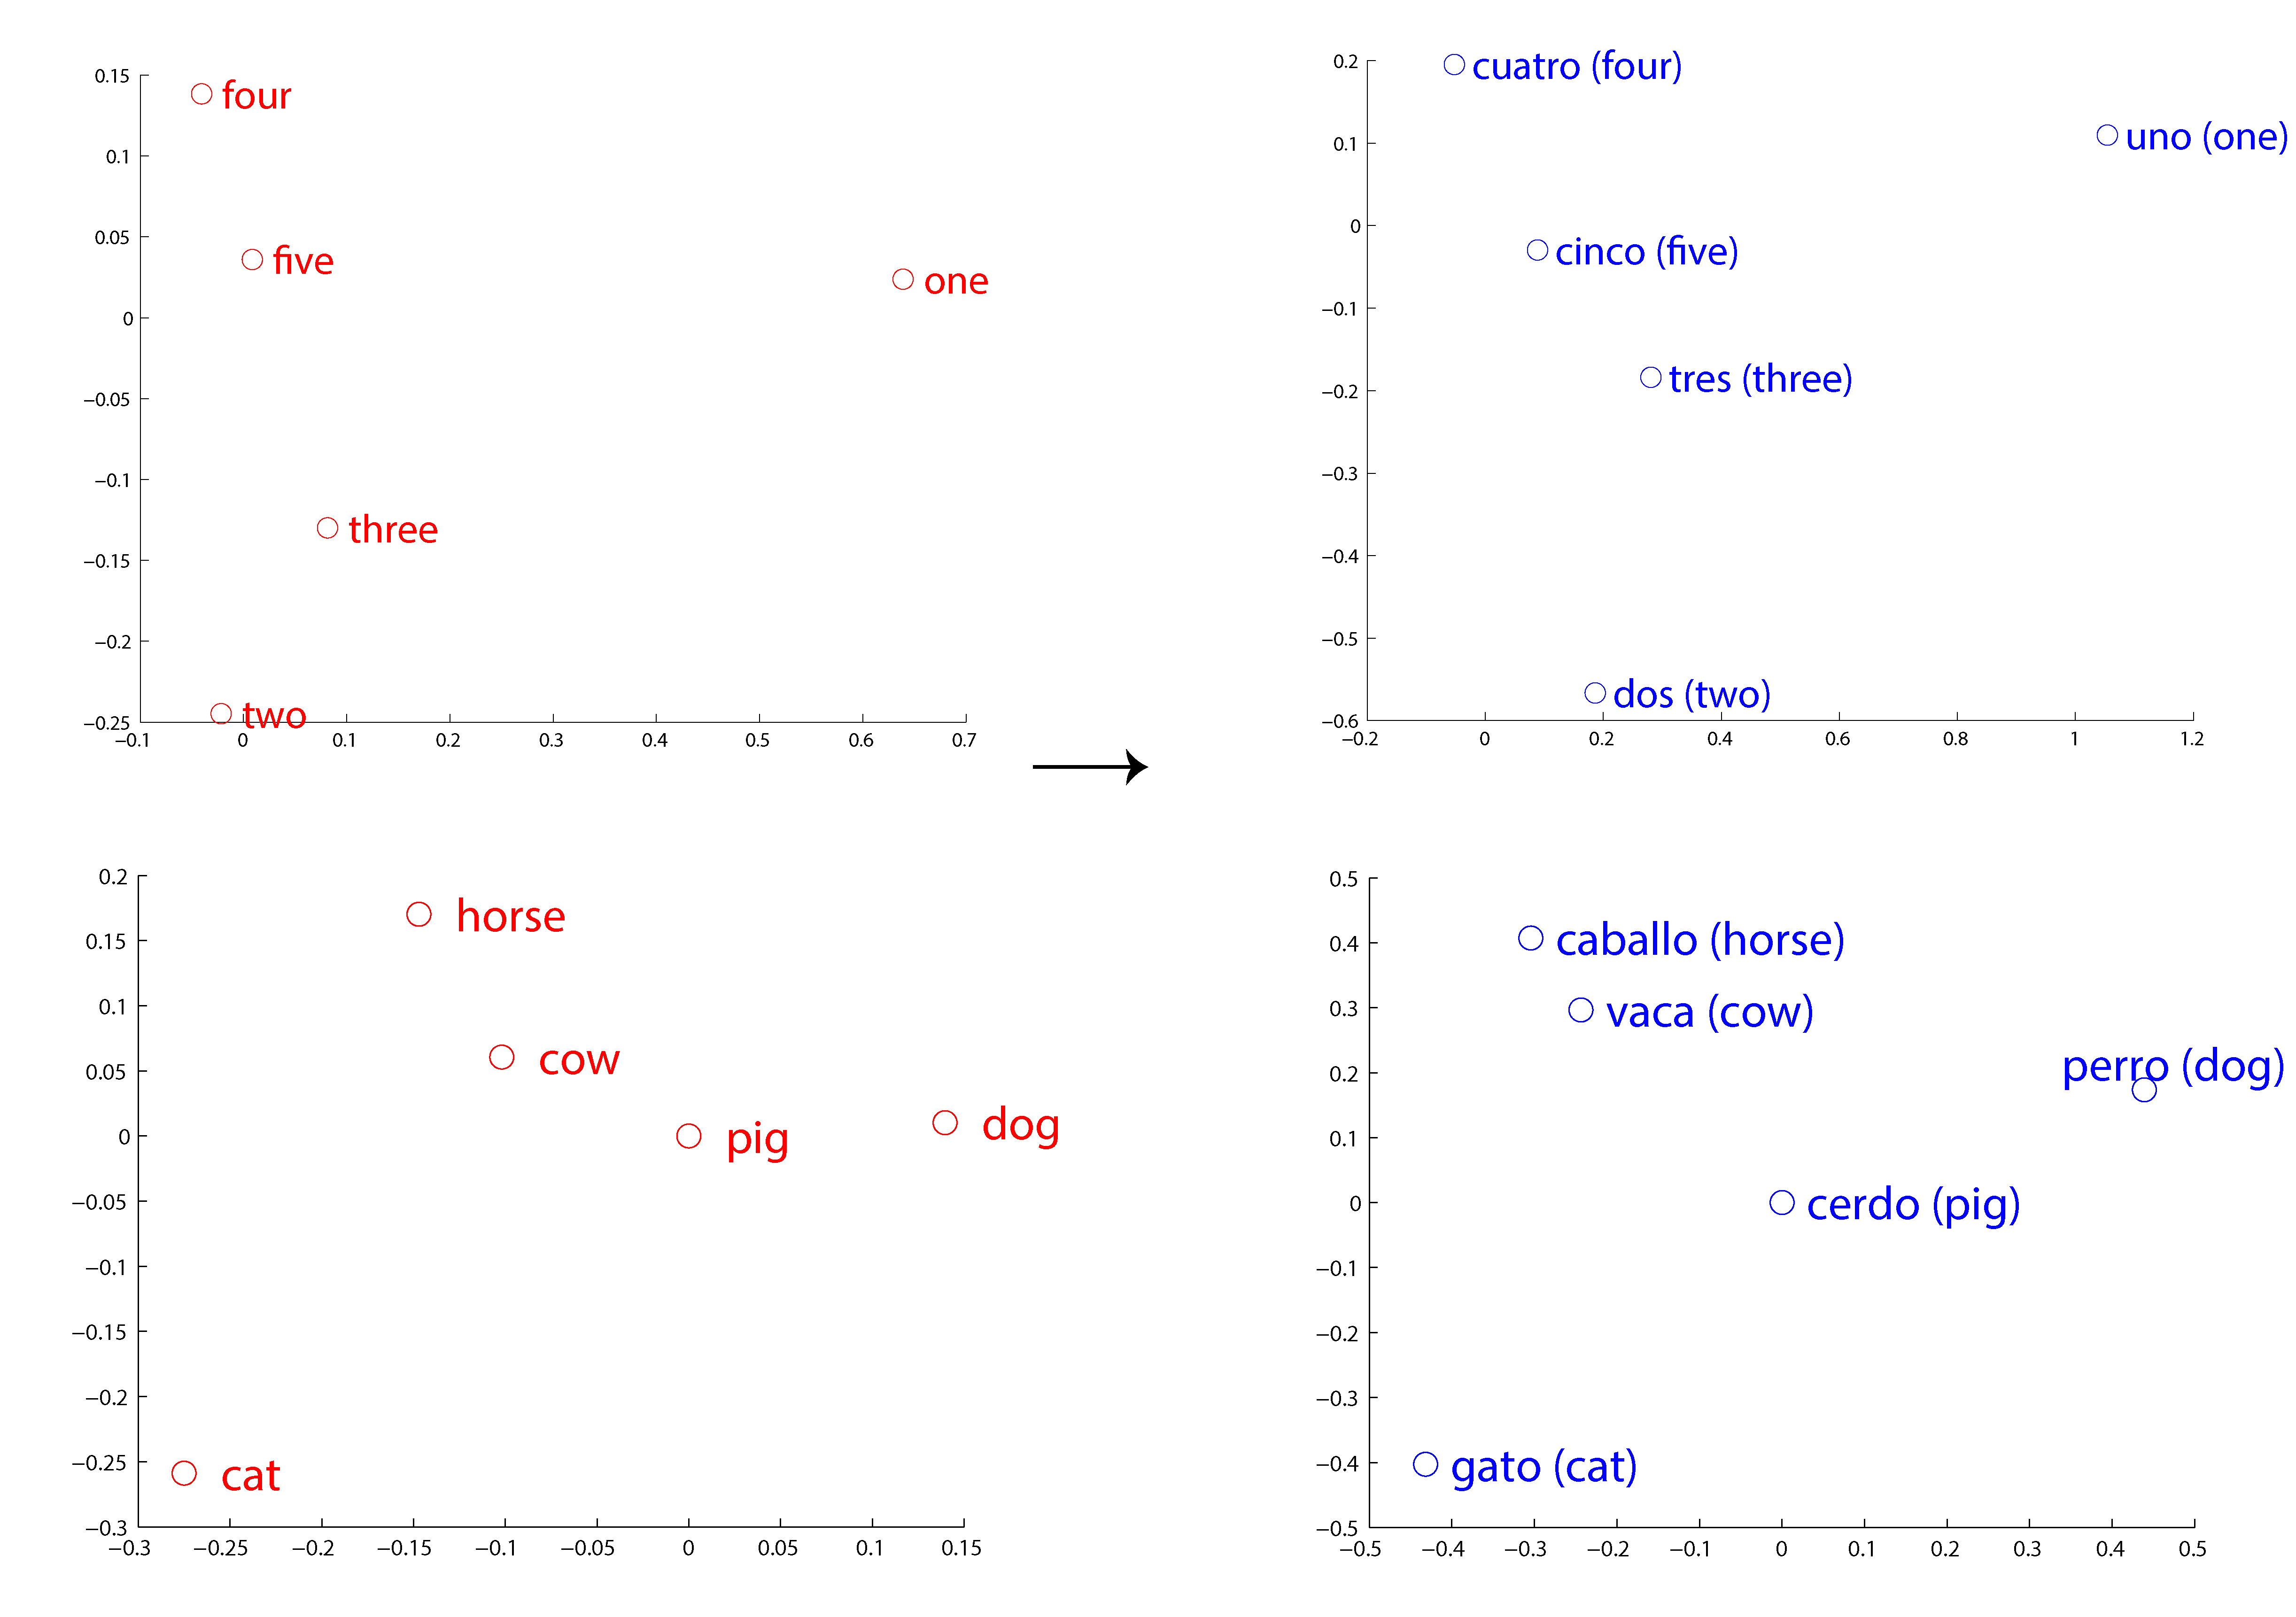
\includegraphics[width=0.8\linewidth,height=10cm,keepaspectratio]{word2vec_translation}
\caption[Word2Vec language translation property]{\textbf{Word2Vec language translation property.}}
\label{fig:w2v_translation}
\end{figure}

The another interesting property is that the the semantically related words are placed close to each other in word vector space, thus forming clusters of semantically related words. It was also observed the word embeddings of similar words in different languages have the same geometrical arrangement in embedding space of respective language. Thus it is also possible to learn linear mapping between different embedding space by vector rotation and scaling \cite{w2v:language_similarities}. Several other regularities can also be captured by performing basic linear operation on word-embeddings \cite{w2v:mikolov_2013_distributed}. 

\section{Echo State Network (ESN)}

Echo State Network (ESN) is a network with a new viewpoint on Recurrent Neural Network (RNN). It is a discrete time continuous state recurrent neural network introduced by Herbert Jaeger \cite{esn:jaeger:2001} and is believed to closely resemble the learning mechanism in biological brains. ESN is found to be computationally simple and inexpensive to process the temporal or sequential data. The main idea of ESN is to operate the random, large, fixed RNN with the input signal and the non-linear response generated by each neuron of the RNN is collectively combined with the desired output signal using regression to learn the output weights \cite{esn:jaeger_tutorial, esn:jaeger:2001,esn:scholarpedia:2007}.

\subsection{ESN Architecture}

ESN is surprisingly efficient variant for RNN training (see fig. \ref{fig:esn_arch}). In the standard RNN all the weights are required to be tuned even-though it was shown that RNN works well enough even without full adaptation of weights. The classical ESN mainly contains three layers, input layer, the hidden layer (also known as reservoir) and the readout layer. The input layer is fully connected to the hidden layer and both the hidden layer and the input layer is connected to the output layer. The output layer is fully connected back to the hidden layer. However the connection from input to output layer and output layer to hidden layer is optional and depends on the task.

The weights from input to reservoir (i.e. $W^{in}$) and from reservoir to reservoir (i.e. $W^{res}$), are sparsely and randomly initialized and more crucially remains untrained during training. The non-zero element in sparse input weight matrix $W^{in}$ and reservoir weight matrix $W^{res}$ are generated from uniform or normal distribution. The weights from the reservoir to output layer (i.e. $W^{out}$) are the only weights learned during supervised training \cite{esn:jaeger:2001, esn:practical_guide}. For ESN approach to work the reservoir should possess the Echo State Property: if a long input sequence is given to the reservoir the reservoir will end up in the same state irrespective of the initial reservoir state. In other word the reservoir states 'echoes' the input sequence and the effect of previous reservoir state and the previous input on the future reservoir states should vanish gradually \cite{esn:practical_guide, esn:jaeger_tutorial}. 

\begin{figure}[hbtp]
\centering
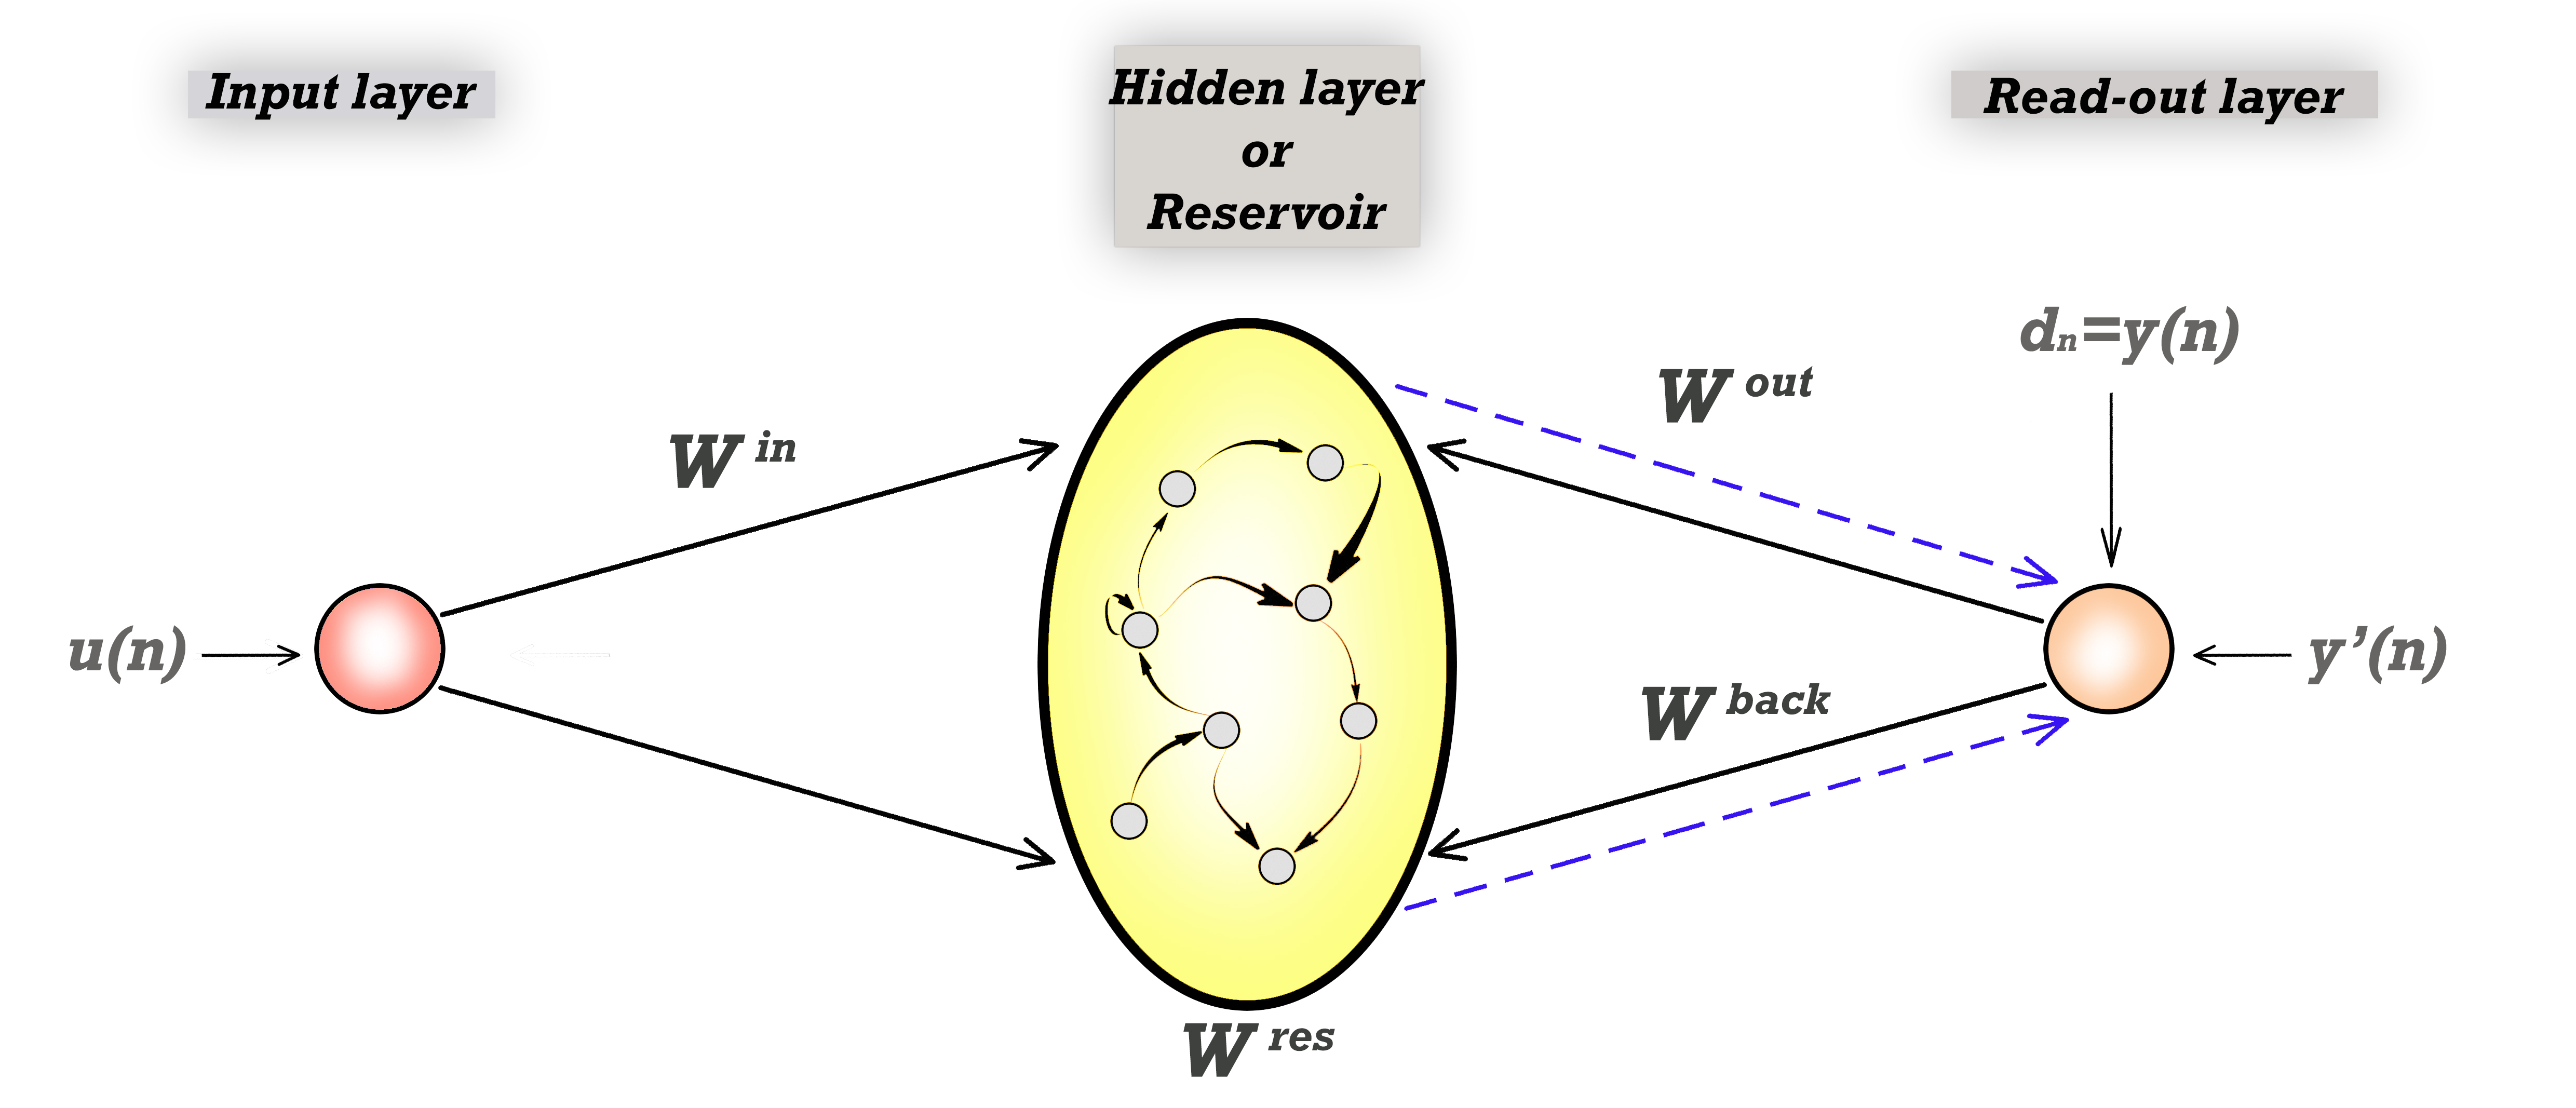
\includegraphics[width=0.8\linewidth]{esn_architecture}
\caption[Architecture of classical ESN]{\textbf{Architecture of classical ESN:} The reservoir is the recurrent neural network with $N_{x}$ units and initialized with random connection. The reservoir is provided input $u(n)$ to the input layer and teacher layer $y(n)$ are pushed output neurons  respectively during training. The input to reservoir weights ($W^{in}$), output neurons to reservoir ($W^{back}$, optional and depends on task) and reservoir to reservoir weight ($W^{res}$) from are also randomly initialized and stays static during learning. The output weight from reservoir to output unit are the only weights learned by the network during training. Adapted from \cite{esn:practical_guide}}
\label{fig:esn_arch}
\end{figure}

To ensure the echo state property in ESN, firstly, the reservoir weights matrix $W^{res}$ and the input weights matrix $W^{in}$ are often generated sparsely (i.e. most of the elements in these matrices will be zero) and randomly from a normal or uniform distribution \cite{esn:practical_guide}. The input weight matrix is however a bit more denser than the reservoir weight matrix. The sparsely generated random reservoir weights matrix $W^{res}$ is often scaled such that its spectral radius $\rho(W^{res})$ i.e. largest absolute eigenvalue, is less than one. To scale the randomly generated $W^{res}$ matrix, it is first divided by its spectral radius and then multiplied with desired spectral radius \cite{esn:jaeger_tutorial}.

\begin{equation}\label{eqn:res_scaling}
W_{new}^{{res}}=\gamma \frac{W^{res}}{\rho(W^{res})}
\end{equation}

where $W_{_{new}}^{{res}}$ is the scaled reservoir weight matrix, $0 < \gamma < 1$ is the desired spectral radius and $\rho(W^{res})$ is the spectral radius of randomly generated reservoir Matrix $W^{res}$.

It is also argued that the $\rho(W^{res}) < 1 $ is not a necessary condition for ESN to have the echo state property and can be achieved even when $\rho(W^{res}) > 1$ \cite{esn:jaeger:2001, esn:practical_guide, esn:jaeger_tutorial}. Intuitively, the spectral radius is a crude measure of the amount of memory the reservoir can hold, the small values meaning a short memory, and the large values a longer memory, up to the point of over-amplification when the echo state property no longer holds. The input weights are also scaled to regulate the non-linearity in reservoir activations. A very high input scaling let the reservoir to behave in highly non-linear manner (because of tanh activation function) whereas a very small input scaling is used wherever linearity is required in a task \cite{esn:practical_guide}.

\subsection{Training ESN}\label{ssec:esn_training}

ESNs are mostly applied supervised machine-learning tasks where temporal or sequentail aspect of the data is to be modeled. Before training, the reservoir of size $N_{x}$, generally containing leaky-integrated discrete-time continuous-value neurons with \textit{tanh} activation function is generated. The reservoir of any computationally affordable size can be used. The bigger the reservoir size, the more the input signal gets non-linearly expanded and easier it will be to find linear combination with the desired output signal \cite{esn:practical_guide, esn:jaeger_tutorial}. With the big reservoir size comes the risk of over-fitting. Thus, It is also important to use proper regularization methods to avoid over-fitting. The reservoir weight $W^{res}$, input weights $W^{in}$ and $W^{back}$ are then randomly initialized.

The training objective of ESN approach is to learn a model which outputs $\textit{y'}$, such that it is as close as possible to the target output \textit{y} by mining the error measure $E(y',y)$ and also generalize well on the data not used for training. Root Mean Square Error is typically chosed as erorr measure E. Thus during training, the given training input signal $\textit{u(n)} \in \mathbb{R}^{N_u}$ and the corresponding teacher signal $\textit{y(n)} \in \mathbb{R}^{N_y}$  is input to the reservoir at every time-step 'n'. Here n = 1,2...,T is the discrete time step for sequence of length T. The reservoir then generate a sequence $\textit{x(n)}$ of $N_{x}$-dimensional reservoir states which is non-linear high dimensional expansion of the input signal $\textit{u(n)}$ \cite{esn:jaeger_tutorial}. The reservoir activation and reservoir state update is computed using following recursive equations:

\begin{equation} \label{eqn:res_update}
x'(n) =\textit {tanh } ( W^{res}x(n-1) + W^{in}.u(n) + W^{back}.y(n-1))
\end{equation}
\begin{equation} \label{eqn:res_state}
x(n) =\textit (1-\alpha) x(n-1) + \alpha x'(n)
\end{equation}

where $\textit{ x(n)}$ is the vector of reservoir neuron's activations and $\textit{ x'(n)}$ is its update at time step $\textit{n}$. \textit{tanh} is reservoir neuron activation function. $ W^{in} \in \mathbb{R}^{{N_x} \times{N_u}}$ and $ W^{res} \in \mathbb{R}^{{N_x} \times{N_x}} $ are input weights and reservoir weights matrices respectively. $ W^{back} \in \mathbb{R}^{{N_x} \times{N_y}} $ is the optional output to reservoir matrix \footnote{this weight matrix is not used in our model implementation}. $\alpha \in (0,1]$ is leaking rate of neurons.  

The leaking rate, $\alpha$, regulates the speed of reservoir update dynamics in discrete time. Smaller value of also induces slow reservoir dynamics thus ensuring the long short-term memory in ESN \cite{esn:practical_guide, esn:optimization_leaky_neurons}. The reservoir activation states are accumulated at every time step for regression with the teacher output. The linear readout weights are then learned using equations:

\begin{equation}\label{eqn:esn_output}
y'(n) = \textit W^{out}x(n)
\end{equation}

where $y'(n) \in \mathbb{R}^{N_y}$ is output of the network and $W^{out} \in \mathbb{R}^{{N_y} \times {N_x}}$ is the output weight matrix.

Writing the equation \ref{eqn:esn_output} in matrix form, the output weights $W^{out}$ are then learned using the following equation:
 
\begin{equation}
Y=W^{out}X
\end{equation}
\begin{equation}
W^{out}=YX^{T}(XX^{T}+{\beta}I)^{-1}
\end{equation}

where $\beta$ is the regularization coefficient parameter of ridge regression and \textit{I} is the Identity matrix. 

Training procedure of ESN, have only few global parameters which are to be optimized: reservoir size $ N_{x} $, spectral radius of $W^{res}$, input scaling of $W^{in}$, leak rate $\alpha$ and the ridge parameter $\beta$. All these parameters can only be optimized by trial and error method and depends heavily on the task under consideration. Usually a grid search is applied to explore the best parameter combination.   
